\section{L'écriture et la langue du carnet}

\subsection{Une cursive rapide}

Hippolyte Combes écrit d'une cursive liée, penchée à droite d'environ trente degrés, à la plume souple : pleins appuyés, déliés fins, finales prolongées en longs traits horizontaux ou plongeants. Les hampes et les jambages, deux à trois fois plus hauts que le corps des lettres, mordent sur les lignes voisines ; les barres de \textit{t}, les points et les accents, posés après coup, glissent vers la droite, si bien que l'accent d'un mot coiffe souvent la lettre suivante et que la barre d'un \textit{t} couvre parfois tout un mot. L'écriture tient en seize à vingt-cinq lignes par page. L'encre change au fil du carnet : violette dans les premiers jours, noire virée au brun d'août à la mi-septembre 1916, de nouveau violette jusqu'en novembre, noire de la fin de novembre à la mi-janvier 1917, violette enfin de la fin de janvier à avril ; quelques comptes sont au crayon. Un changement d'encre au milieu d'une page trahit un ajout postérieur (total d'un compte, mention complémentaire) : l'apparat le signale.

La lecture bute sur trois difficultés récurrentes. Les lettres à jambages (\textit{i, u, n, m, r, v}) se confondent et doivent être comptées une à une. Plusieurs lettres prennent des formes très variables : le \textit{s} monte en haute boucle à l'initiale, descend en \textit{s} long au milieu du mot, plonge en finale ; le \textit{d} rejette sa haste en arrière ; le \textit{r} initial s'orne d'une grande boucle. Enfin certains signes se ressemblent : l'esperluette, qu'Hippolyte Combes trace de cinq ou six manières, se distingue du \textit{y} (tête en V ouvert, descente finissant vers la gauche) et du chiffre 2 bouclé ; la barre oblique du millésime (« /16 ») n'est pas un chiffre 1, et le \textit{f} suscrit des sommes en francs se confond avec un 5. La planche paléographique (fig.~\ref{planche}) réunit des formes caractéristiques ; les lectures douteuses sont discutées, lettre à lettre, dans l'apparat.

\subsection{Abréviations et signes}

L'abréviation est la règle. Les jours de la semaine sont réduits à une ou deux lettres (\textit{Ma.}, \textit{Me}, \textit{J.}, \textit{Ve}, \textit{S.}, \textit{D.}) avant que les formes pleines ne l'emportent en 1917 ; les mots grammaticaux et les adverbes fréquents sont contractés (\textit{ds} « dans », \textit{pr} « pour », \textit{qq} « quelque », \textit{tt}, \textit{tte} « tout, toute », \textit{tjs} « toujours », \textit{s/} « sur », \textit{chz} « chez », \textit{bp} « beaucoup », \textit{lgs} « longs », \textit{merv\textsuperscript{t}} « merveilleusement ») ; les finales sont suscrites (\textit{M\textsuperscript{me}}, \textit{Marg\textsuperscript{te}}, \textit{lieu\textsuperscript{t}}, \textit{Sept\textsuperscript{bre}}). Le signe = vaut « même » (\textit{moi-=}), la croix + « plus » ; les sommes s'écrivent \textit{1\textsuperscript{f} 50}, \textit{75 c}, \textit{84 fr.} Ces formes sont transcrites telles quelles et développées dans l'apparat ; la table des abréviations, en annexe, les réunit.

\subsection{Une langue de notes, mêlée d'anglais}

Le carnet est écrit en style télégraphique : sujets, articles et auxiliaires tombent (\textit{Venu à pied}, \textit{Resté chambre}, \textit{Chevauché matinée entière}), les phrases se suivent par juxtaposition, séparées de tirets. Le vocabulaire anglais du service s'y mêle naturellement, sans marque particulière : \textit{mess}, \textit{breakfast}, \textit{lunch}, \textit{washing}, \textit{food}, \textit{tip}, \textit{groom}, \textit{lorry}, \textit{railhead}, \textit{refilling point}, \textit{green forage}, jusqu'à des hybrides comme \textit{shifterons}. La langue est pourtant celle d'un lettré : notes de couleurs et de lumière, regards d'amateur d'art sur les églises et les beffrois, méditations sur la guerre et sur l'absente. Le glossaire des termes anglais et militaires, en annexe, éclaire ce vocabulaire.

\begin{figure}[p]
\centering
\renewcommand{\arraystretch}{1.05}
\begin{tabular}{@{}p{\dimexpr(\textwidth-6\tabcolsep)/3\relax}p{\dimexpr(\textwidth-6\tabcolsep)/3\relax}p{\dimexpr(\textwidth-6\tabcolsep)/3\relax}@{}}
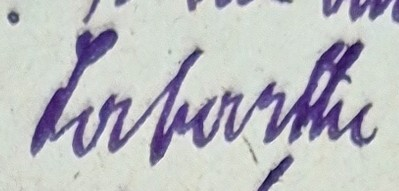
\includegraphics[width=0.96\linewidth,height=12.6mm,keepaspectratio]{illustrations/planche/01_057.jpg} & 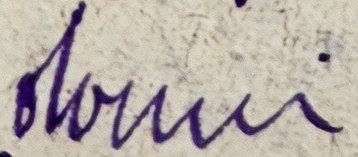
\includegraphics[width=0.96\linewidth,height=12.6mm,keepaspectratio]{illustrations/planche/02_049.jpg} & 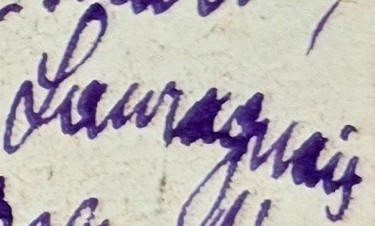
\includegraphics[width=0.96\linewidth,height=12.6mm,keepaspectratio]{illustrations/planche/03_057.jpg} \\
{\scriptsize a fermé, b bouclé — Labarthe \textcolor{LJgris}{(f.~29~r\textsuperscript{o})}} & {\scriptsize d bouclé en arrière — dormi \textcolor{LJgris}{(f.~25~r\textsuperscript{o})}} & {\scriptsize s final plongeant — Lauraguais \textcolor{LJgris}{(f.~29~r\textsuperscript{o})}} \\[1.2mm]
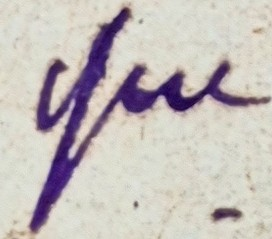
\includegraphics[width=0.96\linewidth,height=12.6mm,keepaspectratio]{illustrations/planche/04_071.jpg} & 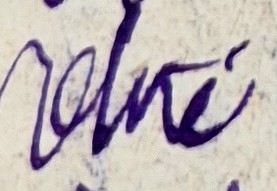
\includegraphics[width=0.96\linewidth,height=12.6mm,keepaspectratio]{illustrations/planche/05_049.jpg} & 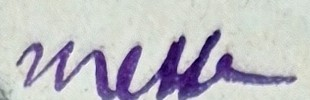
\includegraphics[width=0.96\linewidth,height=12.6mm,keepaspectratio]{illustrations/planche/06_060.jpg} \\
{\scriptsize q à haste droite — que \textcolor{LJgris}{(f.~36~r\textsuperscript{o})}} & {\scriptsize r initial bouclé — retiré \textcolor{LJgris}{(f.~25~r\textsuperscript{o})}} & {\scriptsize ss montants (« ll ») — messe \textcolor{LJgris}{(f.~30~v\textsuperscript{o})}} \\[1.2mm]
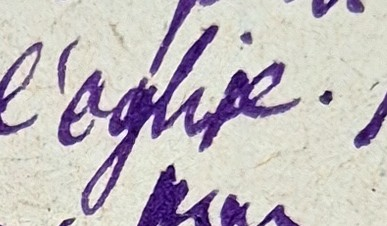
\includegraphics[width=0.96\linewidth,height=12.6mm,keepaspectratio]{illustrations/planche/07_057.jpg} & 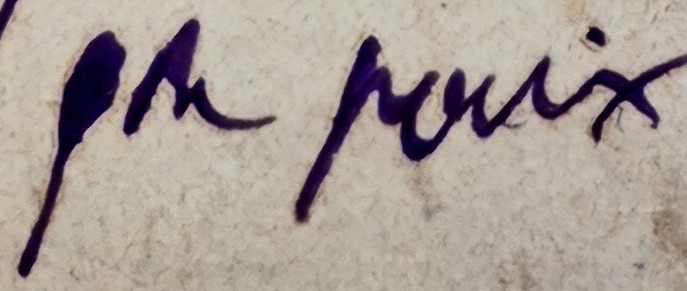
\includegraphics[width=0.96\linewidth,height=12.6mm,keepaspectratio]{illustrations/planche/08_071.jpg} & 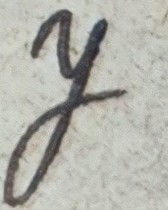
\includegraphics[width=0.96\linewidth,height=12.6mm,keepaspectratio]{illustrations/planche/09_041.jpg} \\
{\scriptsize g et s long descendants — l'église \textcolor{LJgris}{(f.~29~r\textsuperscript{o})}} & {\scriptsize g\textsuperscript{de}, x en croix — gde paix \textcolor{LJgris}{(f.~36~r\textsuperscript{o})}} & {\scriptsize y à tête en V — y \textcolor{LJgris}{(f.~21~r\textsuperscript{o})}} \\[1.2mm]
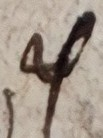
\includegraphics[width=0.96\linewidth,height=12.6mm,keepaspectratio]{illustrations/planche/10_014.jpg} & 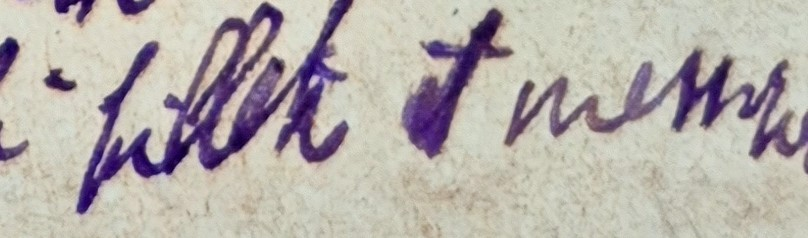
\includegraphics[width=0.96\linewidth,height=12.6mm,keepaspectratio]{illustrations/planche/11_090.jpg} & 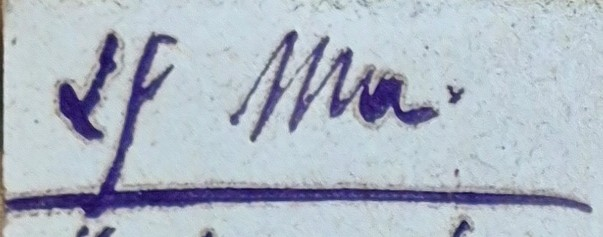
\includegraphics[width=0.96\linewidth,height=12.6mm,keepaspectratio]{illustrations/planche/12_002.jpg} \\
{\scriptsize esperluette « en 4 » — \& \textcolor{LJgris}{(f.~7~v\textsuperscript{o})}} & {\scriptsize \& en « t bouclé » — billets \& mess \textcolor{LJgris}{(f.~45~v\textsuperscript{o})}} & {\scriptsize date soulignée, 5 à drapeau — 25 Ma. \textcolor{LJgris}{(f.~1~r\textsuperscript{o})}} \\[1.2mm]
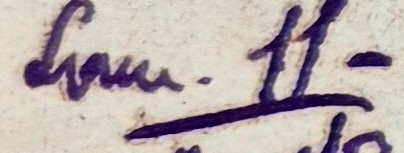
\includegraphics[width=0.96\linewidth,height=12.6mm,keepaspectratio]{illustrations/planche/13_097.jpg} & 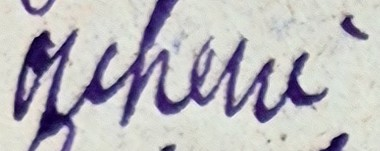
\includegraphics[width=0.96\linewidth,height=12.6mm,keepaspectratio]{illustrations/planche/14_049.jpg} & 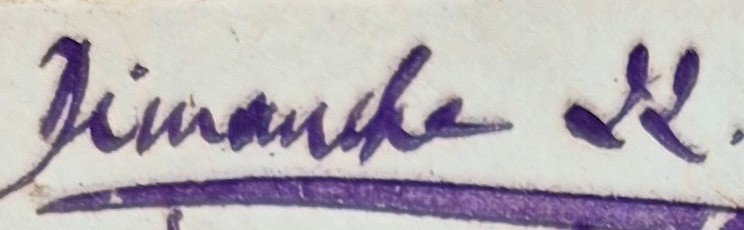
\includegraphics[width=0.96\linewidth,height=12.6mm,keepaspectratio]{illustrations/planche/15_083.jpg} \\
{\scriptsize S en L bouclé, tiret — Sam. 11 — \textcolor{LJgris}{(f.~48~v\textsuperscript{o})}} & {\scriptsize A cursif (a agrandi) — Achevé \textcolor{LJgris}{(f.~25~r\textsuperscript{o})}} & {\scriptsize D en J, 2 bouclé — Dimanche 22. \textcolor{LJgris}{(f.~42~r\textsuperscript{o})}} \\[1.2mm]
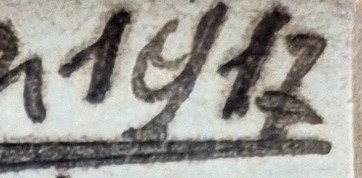
\includegraphics[width=0.96\linewidth,height=12.6mm,keepaspectratio]{illustrations/planche/16_124.jpg} & 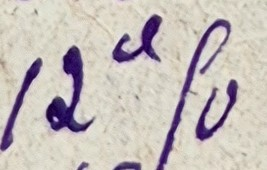
\includegraphics[width=0.96\linewidth,height=12.6mm,keepaspectratio]{illustrations/planche/17_053.jpg} & 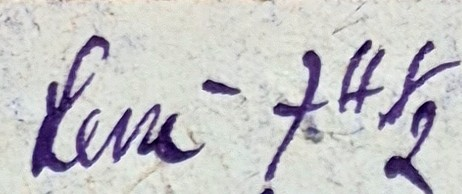
\includegraphics[width=0.96\linewidth,height=12.6mm,keepaspectratio]{illustrations/planche/18_049.jpg} \\
{\scriptsize 7 barré — 1917 \textcolor{LJgris}{(f.~62~r\textsuperscript{o})}} & {\scriptsize f suscrit, 5 bouclé — 12\textsuperscript{f} 50 \textcolor{LJgris}{(f.~27~r\textsuperscript{o})}} & {\scriptsize H suscrit, demi — Levé – 7\textsuperscript{H}\LJfrac{1}{2} \textcolor{LJgris}{(f.~25~r\textsuperscript{o})}} \\[1.2mm]
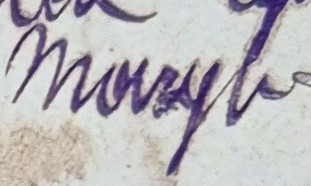
\includegraphics[width=0.96\linewidth,height=12.6mm,keepaspectratio]{illustrations/planche/19_002.jpg} & 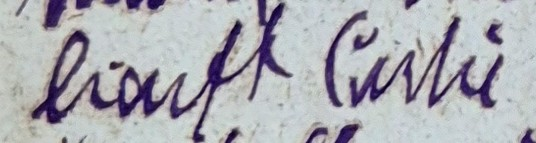
\includegraphics[width=0.96\linewidth,height=12.6mm,keepaspectratio]{illustrations/planche/20_002.jpg} & 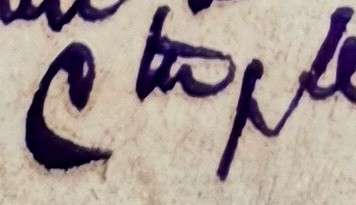
\includegraphics[width=0.96\linewidth,height=12.6mm,keepaspectratio]{illustrations/planche/21_097.jpg} \\
{\scriptsize Marg\textsuperscript{te} (Marguerite) \textcolor{LJgris}{(f.~1~r\textsuperscript{o})}} & {\scriptsize lieut\textsuperscript{t} Curtis \textcolor{LJgris}{(f.~1~r\textsuperscript{o})}} & {\scriptsize C\textsuperscript{tes} p\textsuperscript{les} (cartes postales) \textcolor{LJgris}{(f.~48~v\textsuperscript{o})}} \\[1.2mm]
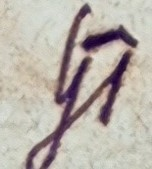
\includegraphics[width=0.96\linewidth,height=12.6mm,keepaspectratio]{illustrations/planche/22_076.jpg} & 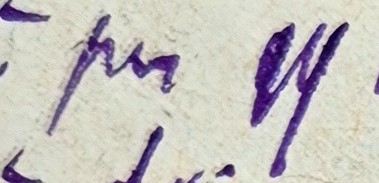
\includegraphics[width=0.96\linewidth,height=12.6mm,keepaspectratio]{illustrations/planche/23_060.jpg} & 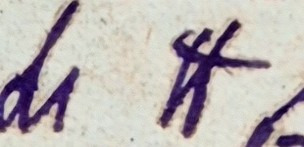
\includegraphics[width=0.96\linewidth,height=12.6mm,keepaspectratio]{illustrations/planche/24_076.jpg} \\
{\scriptsize tjs (toujours) \textcolor{LJgris}{(f.~38~v\textsuperscript{o})}} & {\scriptsize pr (pour) ; qq (quelques) \textcolor{LJgris}{(f.~30~v\textsuperscript{o})}} & {\scriptsize ds (dans) ; tt (tout) \textcolor{LJgris}{(f.~38~v\textsuperscript{o})}} \\[1.2mm]
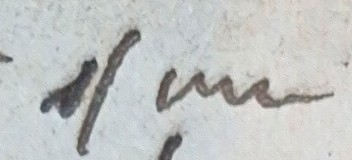
\includegraphics[width=0.96\linewidth,height=12.6mm,keepaspectratio]{illustrations/planche/25_007.jpg} & 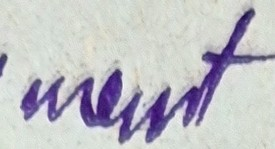
\includegraphics[width=0.96\linewidth,height=12.6mm,keepaspectratio]{illustrations/planche/26_060.jpg} & 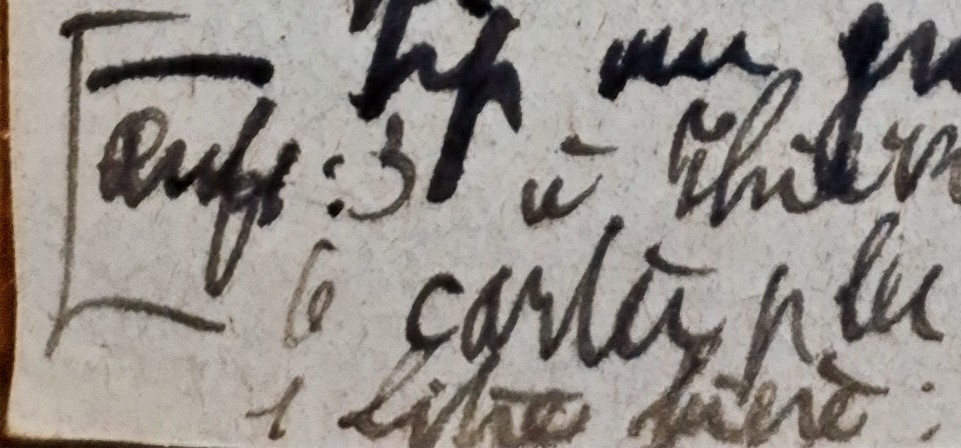
\includegraphics[width=0.96\linewidth,height=12.6mm,keepaspectratio]{illustrations/planche/27_041.jpg} \\
{\scriptsize s/ (sur) — s/ une \textcolor{LJgris}{(f.~3~v\textsuperscript{o})}} & {\scriptsize merv\textsuperscript{t} (merveilleusement) \textcolor{LJgris}{(f.~30~v\textsuperscript{o})}} & {\scriptsize crochet de comptes (3 lignes) \textcolor{LJgris}{(f.~21~r\textsuperscript{o})}} \\[1.2mm]
\end{tabular}
\caption{Planche paléographique : formes caractéristiques de l'écriture d'Hippolyte Combes (1916–1917)}
\label{planche}
\end{figure}
